\documentclass[11pt,a4paper]{article}

\usepackage{amsmath}
\usepackage{amsfonts}
\usepackage{amssymb}
\usepackage{graphicx}
\usepackage{xeCJK}
\usepackage{graphicx}
\usepackage{wrapfig}
\setCJKmainfont[BoldFont=思源黑体 Medium,ItalicFont=方正楷体_GBK]{思源宋体}
\setlength{\parindent}{2em}
\newcommand{\nianfen}[1]{\hspace{-2em}{(#1\textbf{·}\textit{青岛})}}
\usepackage[left=3cm, right=3cm, top=3cm, bottom=3cm]{geometry}
\begin{document}
	\hspace{-2em}{(2018\textbf{·}\textit{原创})
		
	\nianfen{2017}在如图所示电路中,电流表量程为 0~0.6A,电压表量程为 0~3V,电阻$R_2$的阻值为$20$Ω,灯泡$R_1$的阻值和同一电源的电压均保持不变.\textbf{请画出该题的各个等效电路图.}
	\begin{wrapfigure}{r}{0.3\linewidth}
		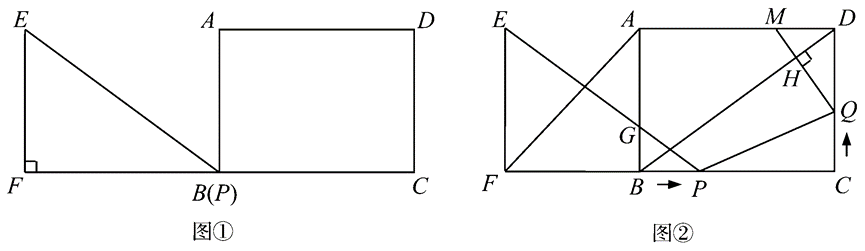
\includegraphics[width=\linewidth]{2017.bmp}
	\end{wrapfigure}
	
	(1)只闭合开关$\rm S_2$、$\rm S_3$时,电流表示数为 0.2A,求电源电压是多少.
	
	(2)只闭合开关$\rm S_1$、$\rm S_2$、$\rm S_3$时,$R_1$正常发光,电路总功率为 2.4W,求$R_1$的阻值是多少.
	
	(3)只闭合开关$\rm S_1$,滑动变阻器$R_3$的滑片调至最右端,$R_3$两端的电压为$U_3$;再将电源更换,保持滑片位置不变,$R_3$两端的电压变为$U_3'$,电流表示数为 0.15A.已知$U_3:U_3'$=$2:3$.求更换电源后,只闭合开关$\rm S_1$、$\rm S_4$时,在不损坏电流表、电压表和灯泡的情况下,$R_3$的阻值变化范围是多少?
	\clearpage
	
	\nianfen{2016}如图甲所示电路,电源电压保持不变.小灯泡L标有“4V 1.6W”字样,滑动变阻器R1的最大阻值为20Ω,定值电阻$ R_2=20Ω $,电流表的量程为0~0.6A,电压表的量程为0~3V.\textbf{请画出该题的各个等效电路图}.求:
	
	\begin{wrapfigure}{r}{0.5\linewidth}
		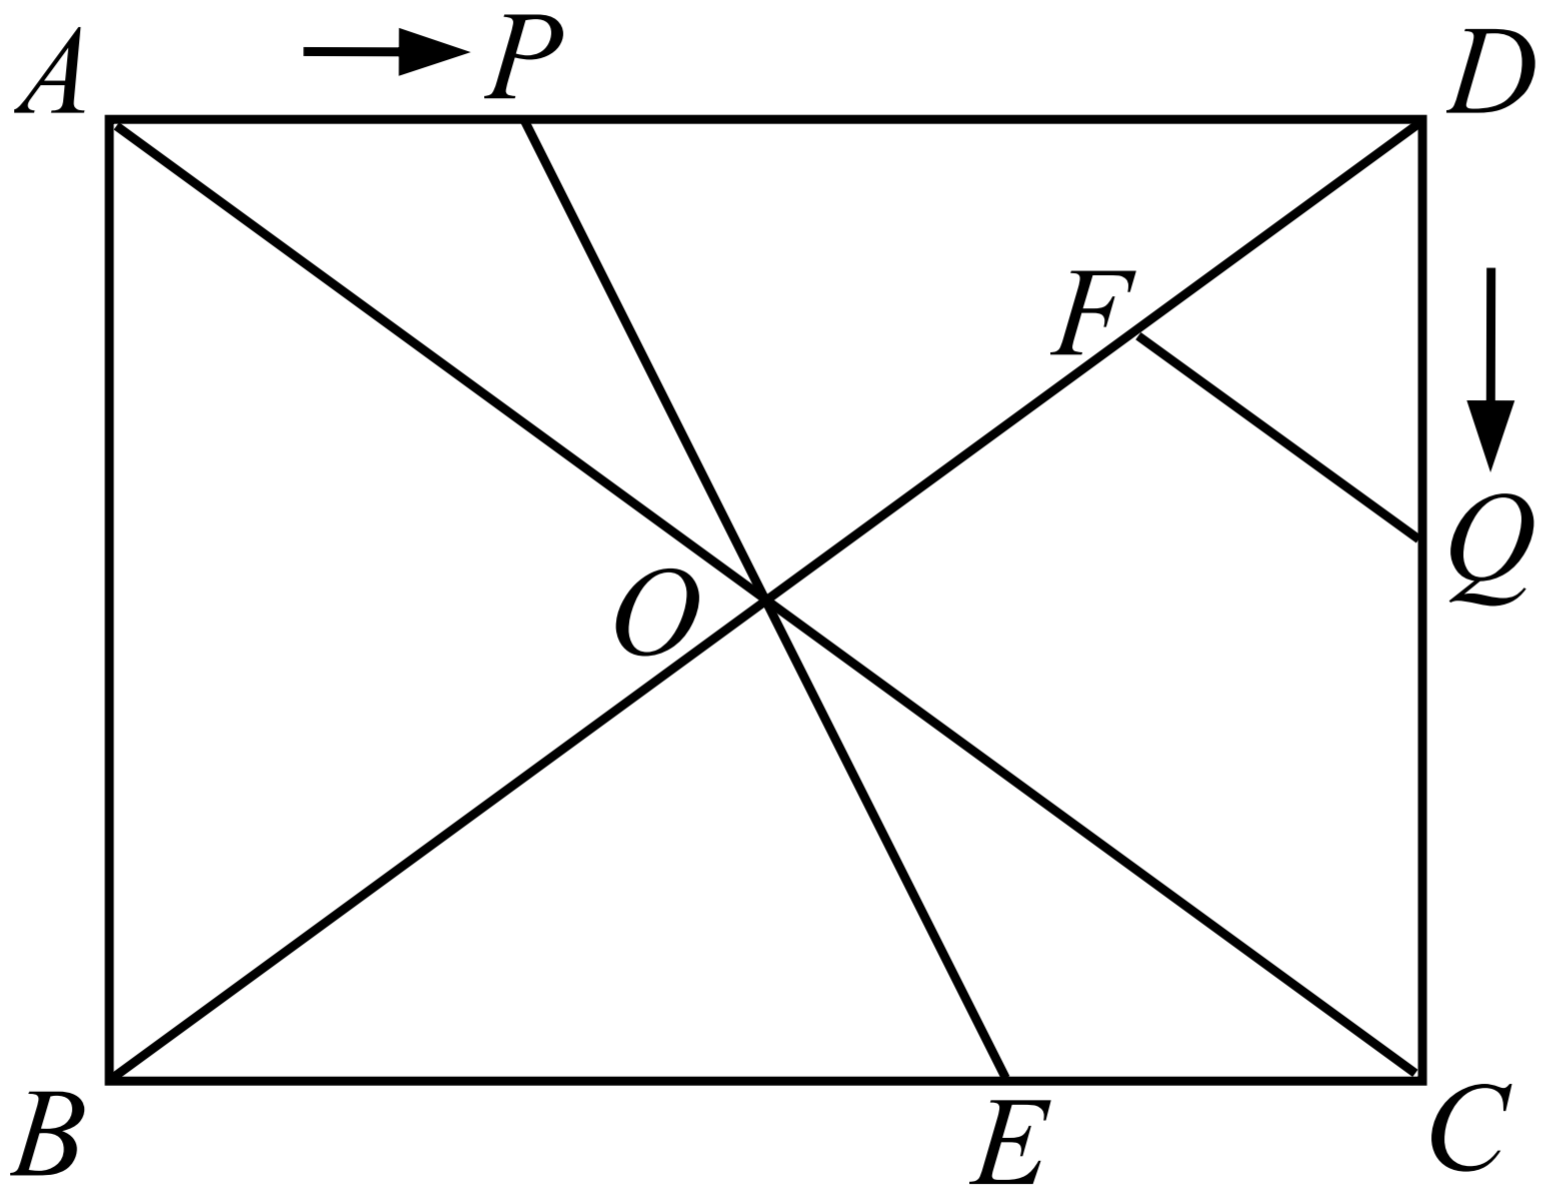
\includegraphics[width=\linewidth]{2016}
	\end{wrapfigure}
	
	(1)小灯泡正常工作时的电阻是多少?
	
	(2)只闭合开关$\rm S $、$\rm S_2 $ 和$\rm S_3 $,移动滑动变阻器$ R_1 $的滑片$ P $使电流表示数为0.5A时,$ R_2 $消耗的电功率为1.25 W.此时滑动变阻器 $ R_1 $接入电路中的阻值是多少?
	
	(3)只闭合开关S和$\rm S_1 $,移动滑动变阻器$ R_1 $的滑片$ P $,小灯泡L的$ I-U $图象如图乙所示.在保证各元件安全工作的情况下,滑动变阻器$ R_1 $允许的取值范围是多少?
	\clearpage
	
	\begin{wrapfigure}{r}{0.3\linewidth}
		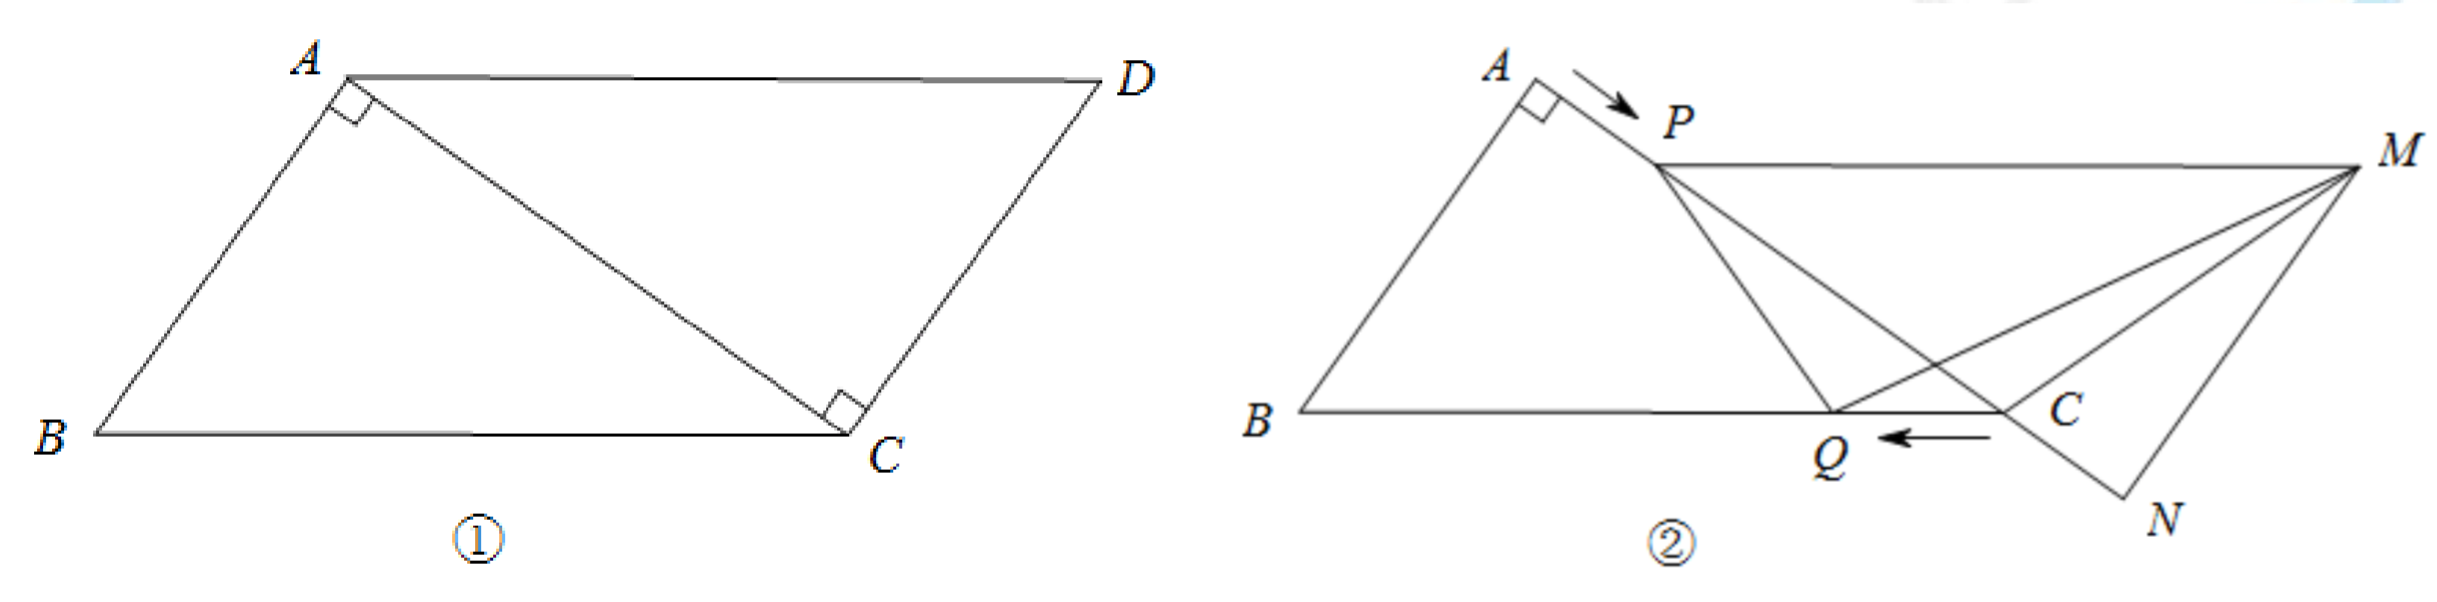
\includegraphics[width=\linewidth]{2015}
	\end{wrapfigure}

	\nianfen{2015}如图所示,电源电压和小灯泡的阻值均保持不变.小灯泡$ R_1 $标有“4V 1.6W”字样,$ R_2=20$Ω,滑动变阻器$ R_3 $允许通过的最大电流为1A,电流表的量程为0~0.6A,电压表的量程为0~3V.\textbf{请画出每个小题的等效电路图}.

	(1)只闭合开关$\rm S_2 $,电压表的示数为2V,则$R_2$消耗的电功率是多少?
	
	(2)在不损毁各元件的情况下,若闭合所有开关,滑动变阻器$R_3$消耗的最大电功率和最小电功率之比为$3:1$;若只闭合$\rm S_3$,小灯泡$R_1$消耗的电功率变化范围是多少?
	\clearpage
	
	\begin{wrapfigure}{r}{0.3\textwidth}
	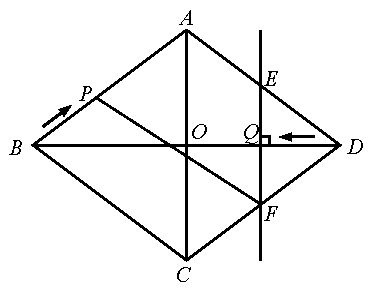
\includegraphics[width=\linewidth]{2014}
	\end{wrapfigure}

	\nianfen{2014}在如图所示的电路中,电源电压和小灯泡的阻值均保持不变,电源电压 $ U=6 $V,小灯泡$ R_2 $标有"6V  3W"字样,电流表的量程为 0~0.6A,电压表的量程为 0~3V,滑动变阻器 $ R_2 $ 的最大阻值为 20Ω,\textbf{请画出该题的各个等效电路图}.
	
	(1)只闭合开关 $\rm S_1 $ 和 $\rm S_2 $ 时,电路消耗的功率为 6W,则闭合开关 $\rm S_1 $、$\rm S_2 $和$\rm S_3 $时,电路的总
	电阻 $ R $=?
	
	(2)在不损坏各元件的情况下,只闭合开关 $\rm S_1 $ 时,$ R_1 $ 消耗的最大功率为 $ P_1 $,只闭合开关$\rm S_2 $时,R2消耗的最小功率为 $ P_2 $,则 $ P_1:P_2= $?
	\clearpage
	
	\begin{wrapfigure}{r}{0.3\linewidth}
		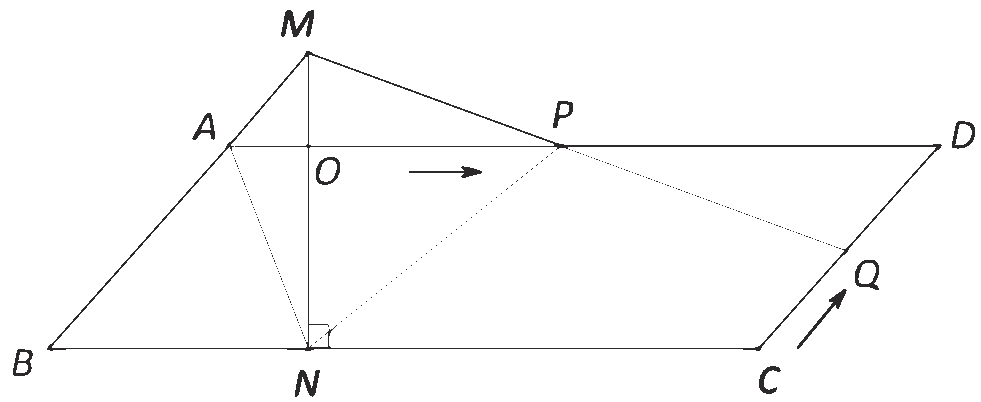
\includegraphics[width=\linewidth]{2013}
	\end{wrapfigure}
	
	\nianfen{2013}在如图所示的电路中,电源电压和各灯泡的阻值均保持不变.电流表的量程为 0~3A,灯泡 $\rm L_1 $ 的电阻 $ R_1=10 $Ω .请画出该题的各个等效电路图.
	
	(1)只闭合开关 $\rm S_1 $、$\rm S_4 $ 时,电流表的示数为 1A.当将滑动变阻器滑片拨至中点处,再将 $\rm S_2 $闭合时,电流表的示数为 1.5A,则在不损坏电流表的情况下,滑动变阻器可以消耗的最大功率与最小功率之比为多少?
	
	(2)只闭合 $\rm S_3 $ 时,电路消耗的最大功率为$ P_1 $;只闭合 $\rm S_4$、 $\rm S_5 $ 时,电路消耗的最小功率为$ P_2 $;只闭合 $\rm S_2 $、$\rm S_3 $、$\rm S_5 $ 时,电路消耗的最小功率为$ P_3 $.已知 $ P_1:P_2:P_3=42:35:30 $,则 $ R_2 $、$ R_3 $ 的限值各为多少?
	\clearpage
	
	\begin{wrapfigure}{r}{0.3\linewidth}
		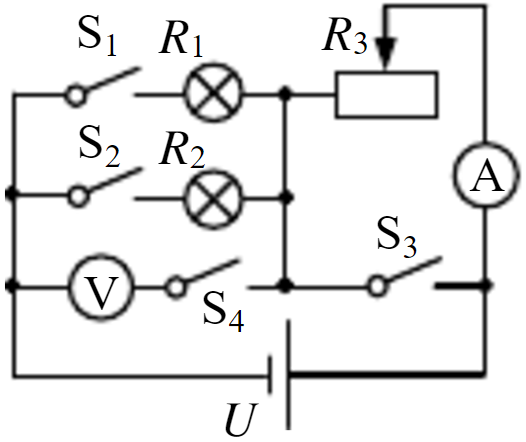
\includegraphics[width=\linewidth]{2012}
	\end{wrapfigure}
	
	\nianfen{2012}在如图所示的电路中,电流表的量程为0~0.6A,电压表的量程为0~15V,电源电
	压$ U=18 $V.灯泡的阻值保持不变.\textbf{请画出每个小题的等效电路图}
	
	(1)闭合开关$\rm S_1 $、$\rm S_3 $时,电路消耗的功率为16.2W,则灯泡$ R_1 $的
	阻值为多少? 
	
	(2)闭合开关$\rm S_1 $、$\rm S_2 $、$\rm S_3 $时,电路消耗的总功率为27W,则灯泡$ R_2 $的阻值为多少?(请写出该小题的解题思路后再求解) 
	
	(3)闭合开关$\rm S_4 $.然后,分别闭合$\rm S_1 $、$\rm S_2 $,在不损坏电流表、电
	压表的情况下,通过调节滑动变阻器,使电路中的电流都达到允许的最大值.这两种情况滑动变阻器消耗的功率之比为多少?
	\clearpage
	
	\begin{wrapfigure}{r}{0.3\linewidth}
		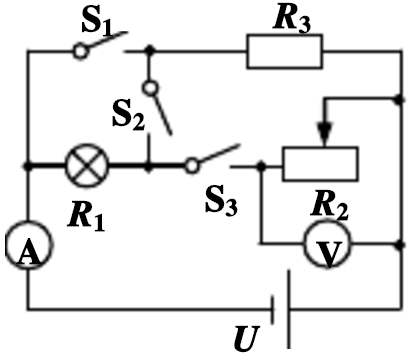
\includegraphics[width=\linewidth]{2011}
	\end{wrapfigure}
	
	\nianfen{2011}在如图所示的电路中,电流表的量程为0~0.6A,电压表的量程为0~3V,$ R_3=4 $Ω.求:\textbf{画出相应的等效电路图}
	
	(1)只闭合开关$\rm S_1 $时,电路消耗的功率为4W,则电源电压$ U= $?
	
	(2)只闭合开关$\rm S_2 $时,灯泡$ R_1 $正常发光,$ R_3 $消耗的功率为0.64W, 则灯泡的电阻$ R_1= $?(写出该小题的解题思路后再求解)
	
	(3)只闭合开关$\rm S_3 $时,在不损坏电流表、电压表和灯泡的情况下,则变阻器$ R_2 $的取值范围是多少?
	\clearpage
	
	\begin{wrapfigure}{r}{0.3\linewidth}
		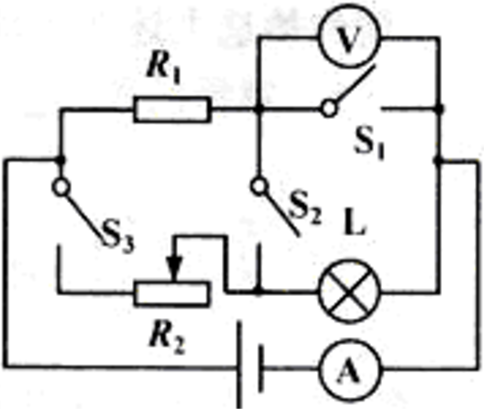
\includegraphics[width=\linewidth]{2010}
	\end{wrapfigure}

	\nianfen{2010}在如图电路中,电源电压为8V,滑动变阻器$ R_2 $的最大阻值为60Ω.电流表的量程为0~0.6A,电压表的量程为0~15V.求:\textbf{求解时画出相应的等效电路图}
	
	(1)只闭合开关$\rm S_1 $时,电流表示数为0.2A.则$ R_1= $?  
	
	(2)只闭合开关$\rm S_2 $时,电压表示数为3.8V.此时小灯泡L正常发光.则小灯泡L的额定功率$ P_{\rm L_{\mbox{\tiny 额}}}= $?
	
	(3)开关$\rm S_1 $、$\rm S_2 $、$\rm S_3 $都闭合时,为保证各电路元件安全使用,则滑动变阻器$ R_2 $的可调范围和电流表相应的变化范围分别是多少?
	\clearpage
	
	\begin{wrapfigure}{r}{0.3\textwidth}
		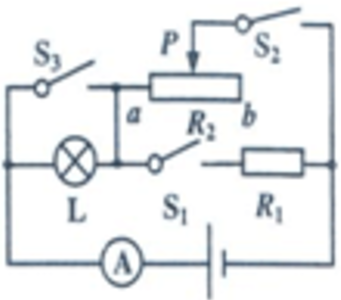
\includegraphics[width=\linewidth]{2009}
	\end{wrapfigure}
	
	\nianfen{2009}如图所示电路,电源电压不变,$ R_1 $=12Ω,小灯泡标有“6V  12W”(电阻不变).求:(画出下列每小题的等效电路图)
	
	(1)只闭合$\rm S_1 $时,电流表示数为0.8A,则电源电压为多大?
	
	(2)当$\rm S_1 $、$\rm S_2 $、$\rm S_3 $都闭合时,将滑片$ P $移动到$ b $端,电流表的示数为1.2A,则滑动变阻器的最大阻值是多少?
	
	(3)只闭合$\rm S_2 $时,移动滑片$ P $,使滑动变阻器所消耗的功率为它最大功率的$\frac{3}{4}$,此时电流表的示数是多少?
	\clearpage
	
	\begin{wrapfigure}{r}{0.25\linewidth}
		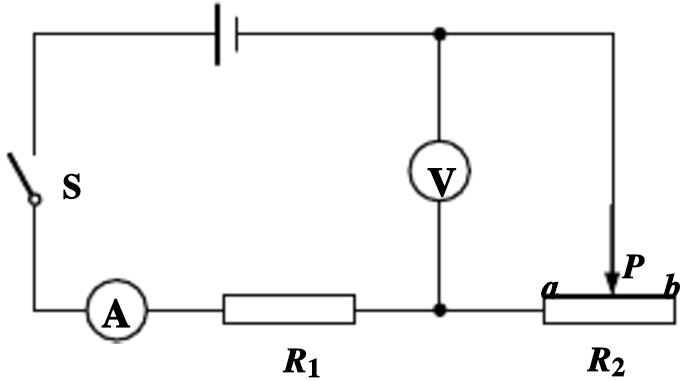
\includegraphics[width=\linewidth]{2008}
	\end{wrapfigure}
	
	\nianfen{2008}如图所示电路,滑动变阻器$ R_2 $的阻值范围为0~15Ω.当滑片$ P $分别移动到$ a $、$ b $两端时,$ R_1 $消耗的功率之比为9:4,滑片$ P $移动到$ a $端时电流表的示数为0.3A.求:
	
	(1) $ R_1 $的阻值
	
	(2)滑片$ P $移动到$ b $端时电压表的示数.
	
	\rule{0em}{15em}
	
	\begin{wrapfigure}{r}{0.3\linewidth}
		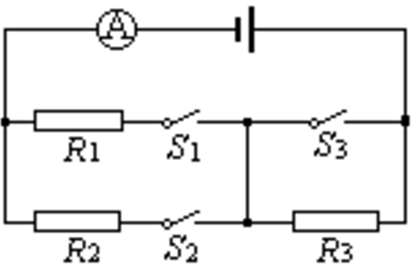
\includegraphics[width=\linewidth]{2007}
	\end{wrapfigure}

	\nianfen{2007}如图所示,电源电压为12V,电阻$ R_1 $=6Ω,只闭合开关$\rm S_1 $时,电路中消耗的总功率为12W;只闻合开关$\rm S_2 $时,电流表的示数变为只闭合$\rm S_1 $时的$\frac{3}{2}$.试求同时闭合开关$\rm S_1 $、$\rm S_2 $、$\rm S_3 $时,通电$ l $min电流做的总功是多少.(请画出等效电路图)
	
	\rule{0em}{10em}
	
	\begin{wrapfigure}{r}{0.35\linewidth}
		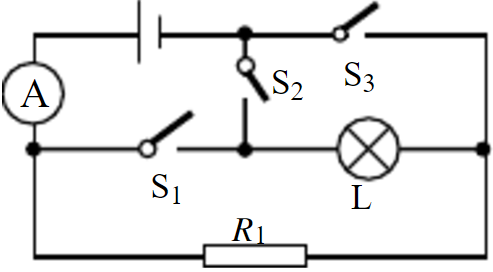
\includegraphics[width=\linewidth]{2006}
		
	\end{wrapfigure}
	
	\mbox{}\\
	
		\mbox{}\\
		
			\mbox{}\\
	
	\nianfen{2006}如图电路中,已知$ R_1 $的阻值是12Ω,当闭合$\rm S_2 $,断开$\rm S_1 $和$\rm S_3 $时,电流表示数是0.5A,灯L的实际功率是其额定功率的$\frac{1}{4}$.当断开$\rm S_2 $,闭合$\rm S_1 $和$\rm S_3 $时,灯L刚好能正常发光. 求灯的额定电压和额定功率.(灯的电阻值保持不变)
	\clearpage
	
	\nianfen{2005}wyy将一个0~16Ω的滑动变阻器和电流表如图甲所示连接在 6V 的电源上,闭合开
	关.请你计算下列问题:
	
	\begin{center}
		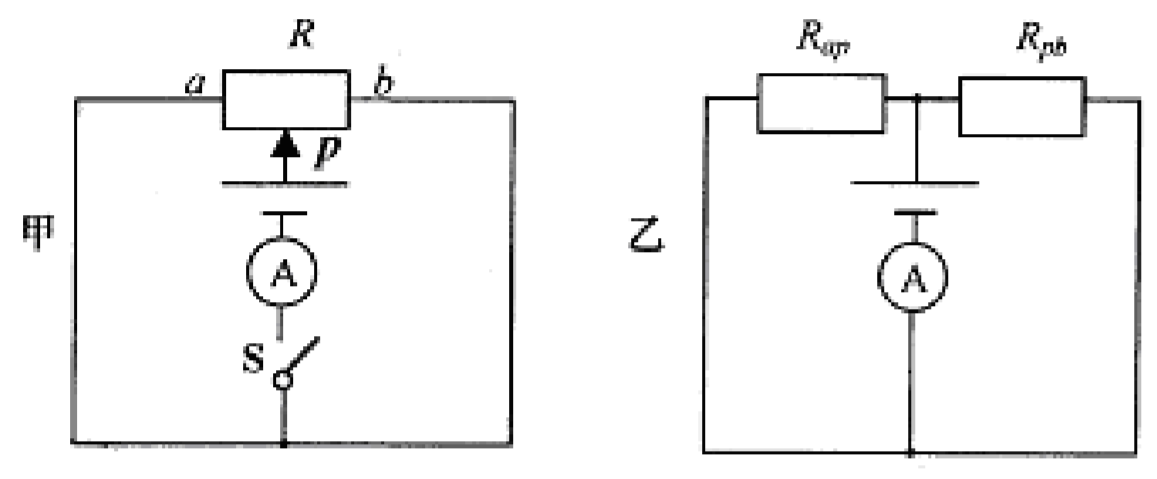
\includegraphics[width=0.7\linewidth]{2005}
	\end{center}
	
	(1)当滑片$  P  $\/置于变阻器中点时,此时等效电路如图乙所示.电路中总电阻是多大?
	
	(2)若电流表量程为 2A ,则当变阻器滑片$  P  $在$ab$之间滑动时,$ R_{ap}  $的阻值变化范围是多少?
	
	\rule{0em}{15em}
	
	\begin{wrapfigure}{r}{0.3\linewidth}
		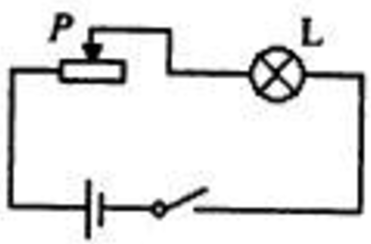
\includegraphics[width=\linewidth]{2004}
	\end{wrapfigure}

	\nianfen{2004}wyy做了一个可以调节亮度的迷你型夜灯,已知小灯泡铭牌是“6V 3.6W”,电池电压为9V,变阻器的变阻范围是
	0~20 ,灯泡的发光效率为30\%.变阻器的电阻调至 多大时,小灯泡实际功率是2.5W?此时小灯泡的发光功率为多大?
	\clearpage
	
	\begin{wrapfigure}{r}{0.3\linewidth}
		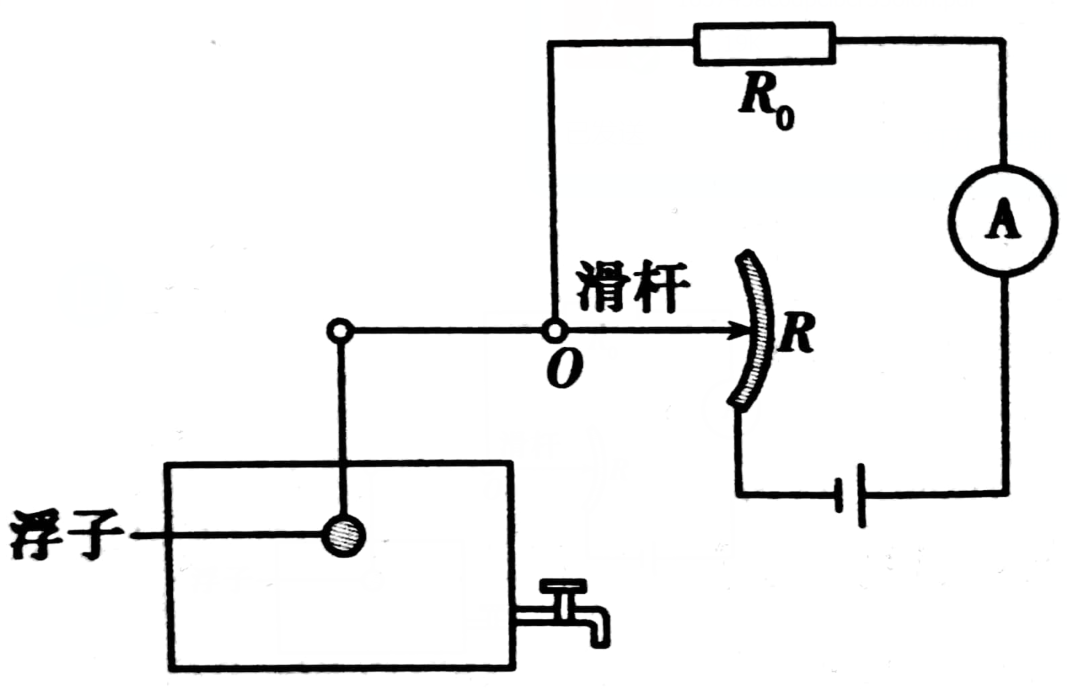
\includegraphics[width=\linewidth]{2003}
		
	\end{wrapfigure}

	\nianfen{2003}右图表示一种自动测定油箱内油面高度的装置.$ R $是滑动变阻器,它的金属滑片是杠杆的一端.当油面最高时,滑动变阻器的滑片恰好在最下端;当油面最低时,滑动变阻器的滑片在最上端.从油量表(由电流表改装而成)指针所指的刻度,可以知道油箱内油面的高度.现已知油的密度$\rho$=0.8×10$^3$kg/m$^3$,浮标的体积是8×10$^{-4}$m$^3$,电源电压是6V,滑动变阻器$ R $的最大阻值是48Ω.求:
	
	(1)当油面的高度是0.4m时,它对油箱底的压强足多少?
	
	(2)若浮标有$\frac{3}{4}$的体积露出油面,它受油对它的浮力是多大?
	
	(3)当油面处在最高处时,电路中电流是0.5A,则串联电阻$ R_0 $的阻值是多大?
	
	(4)当油面处在最低处时,电路中的电流是多大?
	
	\rule{0em}{15em}
	
	\begin{wrapfigure}{r}{0.3\linewidth}
		\includegraphics[width=\linewidth]{2000}
	\end{wrapfigure}
	\nianfen{2000}在实验室中,wyy将一个4欧的电阻和一个6欧的电阻串联起来,接在12伏的电源上,请你替wyy算一算,这两个电阻两端的电压各是多少?要求如下:
	
	(1)写出解题思路.
	
	(2)按上述思路解出此题.
	
	(3)再用另一种思路解出此题.
\end{document}